\chapter{Desenvolvimento Técnico}
Neste capítulo será abordada as técnicas e escolhas de desenvolvimento aplicadas durante o projeto para que o jogo fosse finalizados. Como são os scripts, padrões de projetos e algumas mecânicas e interações presentes em What Weee Are.

\label{desenvolvimento_tecnico}
\section{Scripts}
No moto gráfico Unity, os comportamentos e aspectos ligados às mecânicas do jogo são implementadas via scripts, scripts na linguagem de programação C\#. Scripts atrelados a algum elemento do jogo, devem herdar uma classe chamada MonoBehaviour \footnote{Mais informações \url{https://docs.unity3d.com/ScriptReference/MonoBehaviour.html}} que implementa e nos dá interfaces para adicionar os comportamentos particulares dos elementos do jogo.
Tais scripts são utilizados para implementar aspectos como: movimentação do personagens e inimigos, coleta de itens, emitir eventos após algum acontecimento. Importante atentar a possibilidade de uso de Design Patterns para organizar e mitigar repetições de códigos, alguns padrões de projeto utilizados foram Singleton e Observer.
\subsection{Singleton}
Singleton é uma classe que possui apenas uma instância, possibilitando acesso e controle global. Utilizada para implementar o GameManager, uma classe onde é necessário haver apenas uma única instância, pois é nesta classe que controlamos qual estágio estamos, quais itens coletados, quantas vidas possuí, tempo de jogo. Informações que não pode correr o risco de ter dois ou mais valores.

\subsection{Observer}
Padrão de projeto muito interessante, onde outros objetos observam e aguardam mudanças de outro objeto. Muito importante para implementar casos onde por exemplo, no desmontador de itens, queremos que a cada item depositado nas caixas, queremos testar se algum item mais complexo pode ser gerado. Ou seja, na mudança de estado da caixa de entrada, notificamos o testador de criação. Este padrão nos ajuda a emitir vários eventos à cada mudança, para quem deseja saber das mudanças, tirando a responsabilidade do emissor de saber quem o está observando, a responsabilidade é do objeto interessado de se inscrever para saber das mudanças.

\section{Gerenciador de Diálogos}
No Gerenciador de Diálogos, uma única classe capaz de apresentar os diálogos, imprimindo os parágrafos lentamente e permitindo ir para o próximo parágrafo. Necessitando receber apenas um objeto da classe Dialogue, que contém as frases a serem apresentadas em uma lista, enfileirando todas as sentenças(cada item da lista) do diálogo e imprimindo caractere por caractere, ao finalizar a sentença, inicia a próxima.
\subsection{Dialogo}
Classe Dialogue, implementada para ser capaz de localizar os textos em cada um dos três idiomas(inglês, português e italiano), a quantidade de sentença, as sentenças e quem está apresentando este diálogo.

\break
\section{Inventário}
Implementado para ser capaz de inserir novos itens, adicionar existentes e remove-los quando necessário. Além de a cada operação, os dados são persistidos em formato de arquivo JSON \footnote{Mais informações: \url{https://www.json.org/json-pt.html}} para que o progresso de coleta de itens não seja perdido caso a Unity decida recriar o objeto de Inventário, ou caso o jogo seja finalizado e após um tempo retomado. 
\par
Faz uso de outra estrutura chamada ItemDatabase, sendo responsável por carregar as informações de todos os itens do jogo definidas num arquivo JSON e leva-las ao jogo. Foi uma forma de facilitar a inserção de novos itens ao jogo, sendo necessário apenas adicionar um novo objeto JSON ao arquivo de definição com as informações necessárias para adicionar o item. Possuindo algumas informações necessárias, como identificador único, nome (importante que a imagem do item possua o mesmo nome do item, e esteja localizada em: \url{./Assets/StreamingAssets/Sprites/items/ingame_sprites/}), a descrição, se é isRaw(item primitivo, que não pode ser desmontado), caso falso, necessita a definição de uma lista rawItems, no qual é necessário apontar o identificador do item em que se transforma, e na quantidade. Ver \ref{fig_item_json_definition}.
\begin{figure}[h]
    \centering
    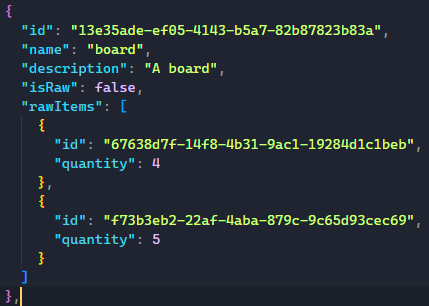
\includegraphics[width=300px]{figuras/item_definition.png}
    \caption{Definição de itens}
    \label{fig_item_json_definition}
\end{figure}


\section{Inimigos}
Os inimigos precisam ser desafiadores e não caírem das plataformas quando chegam em suas bordas, para isso foi implementado um Script chamado AIPatrol, uma inteligência artificial bem simplificada que faz com que os inimigos patrulhem uma área e voltem caso cheguem no fim da plataforma. Fazendo uso de um BoxCollider2D \footnote{https://docs.unity3d.com/Manual/class-BoxCollider2D.html}. Usando um componente adicional que checa se um circulo não visível, que fica a frente do inimigo, deixa de encostar na plataforma.
\begin{figure}[h]
    \centering
    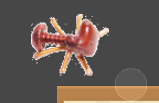
\includegraphics[width=300px]{figuras/GroundChecker.png}
    \caption{Exemplo do Checador de Chão, usado na IA dos inimigos}
    \label{fig_ground_checker}
\end{figure}

